\documentclass[3p,times,12pt]{elsarticle}
\usepackage[utf8]{inputenc}
\usepackage[T1]{fontenc}
\usepackage{graphicx}
\usepackage{amsmath,amssymb}
\usepackage{booktabs}
\usepackage{array}
\usepackage[hypertexnames=false]{hyperref}
\usepackage{microtype}
\usepackage{float}
\usepackage{tikz}
\usetikzlibrary{arrows.meta,positioning,fit,calc,shapes.geometric}
\hypersetup{colorlinks=true,linkcolor=blue,citecolor=blue,urlcolor=blue}
\setlength{\parindent}{0pt}
\setlength{\parskip}{0.8em}
\journal{Deep Learning Course Project}

\begin{document}
\begin{frontmatter}
\title{TrafficVision: Vehicle Detection, Multi-Object Tracking and Calibrated Speed Estimation}
\author{TrafficVision Project Team}
\address{Deep Learning Course Project}
\begin{abstract}
Traffic surveillance requires both reliable vehicle detections and consistent object identities over time. Estimating physical speed adds a separate geometric requirement: image positions must be related to measured points on the road. This report presents TrafficVision, a modular pipeline for vehicle detection, multi-object tracking, polygon-based regions of interest and homography-based speed estimation. The project uses the UA-DETRAC vehicle dataset and provides custom R-CNN-family and compact Transformer-inspired detectors alongside a YOLOv8 baseline. Its published split contains 51 training, 9 validation and 40 test sequences. On the available 10,260-frame validation evaluation, fine-tuned YOLOv8n achieved an AP of 0.750 at IoU 0.50 and 0.564 averaged over IoU thresholds from 0.50 to 0.95; a Faster R-CNN variant with an ImageNet-initialized ResNet-18 backbone achieved 0.719 and 0.507, respectively. These validation results reflect different initializations and training budgets and are not official test-set results. Tracking and metric speed are implemented as downstream components, but the inspected artifacts do not establish tracking benchmark scores or ground-truth speed error. The system therefore reports speed only when a camera-specific metric calibration is available, and its physical accuracy remains to be verified against independent measurements.
\end{abstract}
\begin{keyword}
Vehicle detection \sep multi-object tracking \sep UA-DETRAC \sep homography \sep speed estimation \sep deep learning
\end{keyword}
\end{frontmatter}

\section{Introduction}
\label{sec:introduction}
Traffic cameras can support vehicle monitoring without installing a separate detector for every lane. A useful system must identify vehicle locations in individual frames, maintain identities through motion and partial occlusion, and express any speed estimate in physical units. These tasks are related, but a bounding box or a track identity alone does not establish how many metres the vehicle has travelled.

Object detectors offer complementary accuracy and computational trade-offs. Region-based detectors use proposals and region features, while one-stage detectors predict objects more directly. Transformer-based detection uses a set of object queries and assignment-based training. These families provide useful comparisons on traffic footage, particularly for distant vehicles and crowded scenes \cite{rcnn,fast,faster,rtdetr}. In a tracking-by-detection system, the detector's missed and low-confidence observations also affect trajectory continuity \cite{bytetrack}.

We present TrafficVision, a course project that connects a selection of detectors to interchangeable trackers and a camera-specific measurement pipeline. Its principal components are: (1) a UA-DETRAC annotation parser and sequence-level split; (2) custom detectors and a pretrained YOLOv8n baseline; (3) tracking and polygon zones; and (4) projection onto a road plane followed by speed estimation. The implementation, configurations and available experiment artifacts are published in the project repository on Hugging Face \cite{repository}.

This report distinguishes implemented capabilities from measured outcomes. We analyse the available \emph{validation} detection results and describe the downstream tracking and speed pipeline without treating the existence of an implementation as a quantitative validation. Reproduction of the complete experiment, a held-out test comparison and physical speed verification require the additional evidence listed in Section~\ref{sec:limitations}.

\section{Dataset and Preprocessing}
\label{sec:dataset}
\subsection{UA-DETRAC}
UA-DETRAC is a benchmark for vehicle detection and tracking in road-camera footage, with bounding boxes, trajectory identifiers and vehicle attributes \cite{detrac}. The project uses four foreground classes: \texttt{car}, \texttt{bus}, \texttt{van} and \texttt{others}; label zero is reserved for detector background. Images are associated with their sequence and one-based frame number. The parser converts annotation boxes from left/top/width/height to continuous $(x_1,y_1,x_2,y_2)$ coordinates and retains track IDs and ignored regions \cite{architecture}.

\subsection{Sequence-level split}
To reduce leakage between adjacent video frames, complete sequences are assigned to only one split. Table~\ref{tab:splits} reports the published manifest counts rather than assuming a random frame-level division \cite{manifest}. These are project split counts and are not, by themselves, a claim of compliance with every official UA-DETRAC evaluation setting.
\begin{table}[htbp]
\centering
\caption{Published sequence and frame counts.}
\label{tab:splits}
\begin{tabular}{lrr}
\toprule
Split & Sequences & Frames \\
\midrule
Training & 51 & 71,825 \\
Validation & 9 & 10,260 \\
Test & 40 & 56,167 \\
\midrule
Total & 100 & 138,252 \\
\bottomrule
\end{tabular}
\end{table}

The repository contains a local frame manifest, a sequence split and TAR shards for remote data access. Training can read local data or use streaming/cache sources; the selected mode and storage environment should be recorded when reproducing an experiment \cite{repository}. In the published YOLO training configuration, \texttt{yolo\_stride: 5} is specified for train and validation export. Thus the YOLO training input should not be described as every frame of the full training split without checking the exported dataset \cite{yoloconfig}.

\subsection{Ignored regions and class mapping}
The shared evaluator removes predictions whose box centres fall inside ignored rectangles, except when a prediction matches a labelled positive of the same class at IoU at least 0.5. This project-specific rule must accompany the metrics when comparing results \cite{evaluationcode}. The COCO-pretrained YOLO baseline maps car to car, bus to bus and truck to \texttt{others}; COCO provides no corresponding pretrained \texttt{van} category in this mapping. The fine-tuned checkpoint uses the four UA-DETRAC labels. This difference limits a direct interpretation of per-class baseline results.

\section{Methodology}
\label{sec:methods}
\subsection{System overview}
The pipeline separates detection, tracking, region assignment, geometry and export. For each video frame, a detector produces boxes, class labels and confidence scores in original-image coordinates. An interchangeable tracker associates observations across frames and emits object IDs. A polygon manager can retain road regions, assign near/far zones and apply zone-specific confidence thresholds. The bottom-centre of a tracked box is then used as an approximate road-contact point. If a valid camera calibration is available, that point is projected to a metric road plane and passed to a per-track speed estimator. The resulting frames and trajectories can be exported as MP4, CSV and JSON \cite{architecture}.

Figure~\ref{fig:pipeline} separates the detector and association steps from physical calibration. Zone filtering is applied to detections before association; tracked boxes are then assigned to zones for downstream measurement. Camera-specific geometry and valid timing are needed only for the metric branch.
\begin{figure}[htbp]
\centering
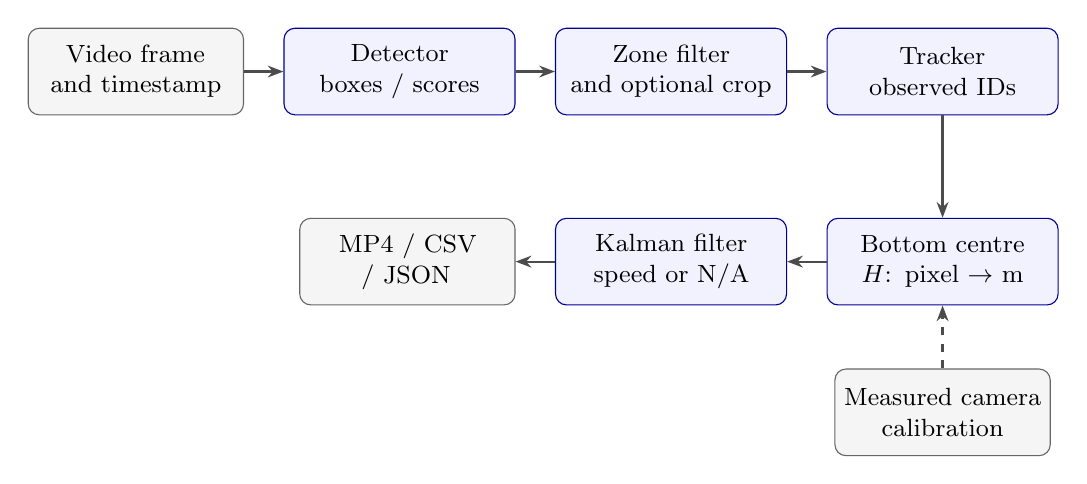
\begin{tikzpicture}[
 node distance=5mm and 5mm,
 block/.style={draw=blue!60!black,rounded corners,fill=blue!5,minimum height=11mm,align=center, text width=27mm,font=\small},
 io/.style={draw=black!60,rounded corners,fill=black!4,minimum height=11mm,align=center,text width=25mm,font=\small},
 arrow/.style={-{Stealth[length=2mm]},thick,draw=black!70}]
\node[io] (video) {Video frame\\and timestamp};
\node[block,right=of video] (detect) {Detector\\boxes / scores};
\node[block,right=of detect] (zone) {Zone filter\\and optional crop};
\node[block,right=of zone] (track) {Tracker\\observed IDs};
\draw[arrow] (video) -- (detect); \draw[arrow] (detect) -- (zone); \draw[arrow] (zone) -- (track);
\node[block,below=13mm of track] (project) {Bottom centre\\$H$: pixel $\to$ m};
\node[block,left=of project] (speed) {Kalman filter\\speed or N/A};
\node[io,left=of speed] (export) {MP4 / CSV\\/ JSON};
\node[io,below=8mm of project] (cal) {Measured camera\\calibration};
\draw[arrow] (track) -- (project); \draw[arrow] (project) -- (speed); \draw[arrow] (speed) -- (export);
\draw[arrow,dashed] (cal) -- (project);
\end{tikzpicture}

\caption{TrafficVision data flow. Solid arrows denote the data path; speed is emitted only when camera calibration and sufficient valid observations are available. Diagram drawn for this report from the published code.}
\label{fig:pipeline}
\end{figure}

\subsection{Vehicle detection}
\textbf{R-CNN and Fast R-CNN.} Both configurations use external region proposals. In the project R-CNN variant, proposals are cropped and processed individually by a convolutional network. The class and box heads are trained jointly with a softmax classifier; this differs from the original multi-stage SVM-based R-CNN procedure \cite{rcnn}. Fast R-CNN shares image-level convolutional features and extracts region features for classification and regression, following the shared-feature motivation of Fast R-CNN \cite{fast}. Selective Search is used as the configured proposal strategy in these experiments.

\textbf{Faster R-CNN.} The project assembles a backbone, anchor generator, region proposal network, RoI Align, classification head and bounding-box regressor using reusable Torchvision operations. One experiment initializes a compact convolutional backbone from scratch, while a second initializes a ResNet-18 backbone with ImageNet weights. The latter is transfer learning, not a fully scratch-trained detector \cite{faster,architecture}. The backbone and parameter count change together, so this comparison cannot isolate the effect of pretraining alone.

\textbf{Compact RT-DETR-inspired detector.} The custom Transformer variant combines multiscale CNN features, an attention-based hybrid encoder, cross-scale fusion, top-$k$ query selection, iterative decoder layers and Hungarian matching with classification and box losses. It uses dense cross-attention and omits denoising queries and other details of the official RT-DETR implementation. Accordingly, its scores must not be presented as a reproduction of the published RT-DETR benchmark \cite{rtdetr,rtdetrcode}.

\textbf{YOLOv8n baseline.} The repository includes a COCO-pretrained YOLOv8n baseline and a UA-DETRAC fine-tuned checkpoint. The baseline and fine-tuned variant share the YOLO family but have different class spaces and training histories. We evaluate them with the project detection evaluator rather than treating the baseline's COCO labels as identical to the target label set \cite{yolo,evaluationcode}.

\subsection{Tracking and polygon zones}
The tracker adapter accepts normalized detections from any supported detector. The available choices include a SORT variant based on Kalman motion prediction and IoU association, ByteTrack, and BoT-SORT. ByteTrack uses low-confidence detections in an additional association stage, which can help reconnect an existing track when object confidence drops \cite{sort,bytetrack,botsort}. These adapters provide a common interface; their presence alone does not establish the tracking accuracy of a particular detector--tracker pair.

Polygon zones define areas of interest in image coordinates. Zone assignment uses the box bottom-centre, and configured far-zone crops can be processed separately before boxes are mapped back and merged. A polygon can filter or organize detections, but it does not create missed detections or guarantee identity recovery. Zone geometry and resolution must match the individual camera.

\subsection{Projection and speed}
For an image point $(u,v)$ on the approximately planar road, a camera-specific homography maps it to world coordinates in metres:
\begin{equation}
\lambda\begin{bmatrix} X & Y & 1 \end{bmatrix}^{\!T} =
H\begin{bmatrix} u & v & 1 \end{bmatrix}^{\!T}.
\end{equation}
At least four corresponding non-collinear points are required to estimate the transformation, but their physical coordinates must come from real measurements. The calibration should be checked using independent points not used for fitting \cite{opencvhomography}. Projecting a bottom-centre box point is an approximation: occlusion and low camera angles can shift it away from the true road-contact point.

For observations separated by elapsed time $\Delta t$, a simple displacement-based speed is $v_{\mathrm{km/h}}=3.6\lVert\Delta(X,Y)\rVert/\Delta t$. The video pipeline uses a constant-velocity Kalman estimator on projected positions; measurement uncertainty is propagated using the homography Jacobian. It can suppress output for short or uncertain tracks and reject incompatible observations. Actual timestamps or a valid constant frame rate are essential, including across gaps. Without a reliable metric calibration, speed remains \texttt{N/A}; UA-DETRAC bounding boxes and IDs alone are not ground-truth vehicle speeds \cite{architecture}.

\section{Detector Architectures and Learning Objectives}
\label{sec:detector-details}
This section explains the detector families and their project-specific implementation choices. The models share an output contract, but their internal feature extraction and proposal mechanisms differ. The published comparison should be read as an evaluation of the actual configurations, not as a general ranking of the corresponding papers.

\subsection{Bounding boxes, class labels and intersection over union}
An image with width $W$ and height $H$ contains zero or more objects. A ground-truth object is represented by a foreground label $c\in\{1,2,3,4\}$ and a bounding box $b=(x_1,y_1,x_2,y_2)$. The detector produces a set of predicted boxes, labels and confidence scores. Predictions and targets must refer to the same original image coordinate system before evaluating or tracking. Resizing, cropping and padding are internal processing operations; the outputs supplied to the tracker must be mapped back.

For two boxes $A$ and $B$, intersection over union (IoU) measures their overlap:
\begin{equation}
\operatorname{IoU}(A,B)=\frac{|A\cap B|}{|A\cup B|}.
\end{equation}
The intersection has zero area when boxes do not overlap. IoU is independent of class: a detector evaluation additionally requires matching class labels. High IoU indicates similar spatial extent but does not establish that two observations at different times belong to the same vehicle.

One-stage and region-based detectors may produce multiple boxes around the same object. Non-maximum suppression (NMS) normally ranks predictions by score and removes sufficiently overlapping lower-scoring boxes within a class. NMS can suppress duplicate responses, but an aggressive threshold can also remove adjacent vehicles in dense traffic. Query-based set prediction instead encourages one-to-one assignments during training; implementation details still determine how many queries and scores are returned.

\subsection{R-CNN: region-wise feature extraction}
R-CNN introduced the idea of applying a convolutional network to candidate regions rather than designing a separate hand-crafted feature extractor for every object category \cite{rcnn}. A proposal algorithm first generates many candidate rectangles. Each candidate is cropped, transformed to a standard input size and sent through a CNN. A classifier scores foreground classes and background, while a regression component adjusts the predicted box.

The project uses this \emph{region-wise computation pattern}, not the complete original R-CNN training recipe. The network processes individual proposal crops and uses a jointly trained softmax classification and box-regression head. The published scratch configuration uses a small convolutional backbone and up to 100 proposals. No SVM training stage is claimed for this implementation. Selective Search creates the candidate regions outside the learned network, so proposal generation and repeated crop processing add latency.

The pipeline is useful pedagogically: it exposes the relationship between proposal quality, classification and localization. Its drawbacks are equally important. If proposal generation misses a small vehicle, the classifier cannot recover it. Overlapping candidate crops repeat substantial CNN work, and feature extraction cost grows with the number of proposals. A tight proposal budget may improve runtime while reducing proposal recall. These effects should be measured rather than inferred solely from the training loss.

\subsection{Fast R-CNN: shared convolutional features}
Fast R-CNN improves the region-based workflow by running the backbone once over the image. Proposed boxes are mapped to a shared feature map, and a region-of-interest operation converts each variable-size region into a fixed-size feature tensor. The region head then predicts class scores and box corrections \cite{fast}. This reduces repeated backbone work while retaining external proposal generation.

The TrafficVision implementation uses RoI Align through Torchvision components and shares the image-level features for its classification and box heads. In the published configuration, Selective Search remains external and the proposal budget is 300. Thus the backbone is shared, but the proposal stage is not a learned region proposal network. Selective Search can still dominate total latency, especially on larger input images.

For illustration, a standard multi-task region-head objective can be expressed as
\begin{equation}
L_{\mathrm{roi}}=L_{\mathrm{cls}}(p,c)+\mathbb{1}[c>0]\,\lambda L_{\mathrm{box}}(t,t^*),
\end{equation}
where $p$ is the class distribution, $c$ is the assigned label, $t$ is the predicted box parameterization and $t^*$ is its regression target. Box regression applies to foreground assignments; background regions contribute to classification. This equation explains the general role of the two heads and does not assert a particular numerical value of $\lambda$ for every detector in this project.

\subsection{Faster R-CNN: learned proposals}
Faster R-CNN replaces the separate proposal generator with a region proposal network (RPN) operating on shared convolutional features \cite{faster}. At each feature-map location, anchors of several sizes and aspect ratios act as candidate reference boxes. The RPN predicts objectness and box adjustments; proposed regions then enter an RoI head for final classification and regression. The broad structure is illustrated in Fig.~\ref{fig:faster}.

\begin{figure}[htbp]
\centering
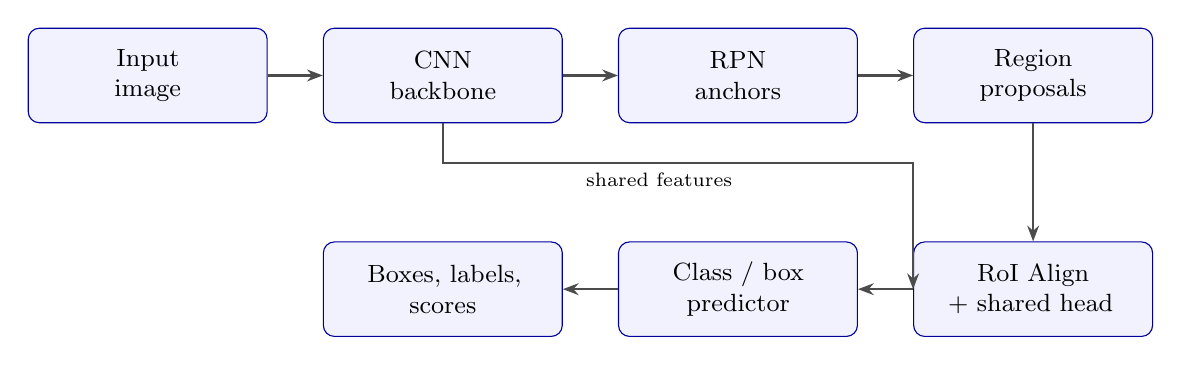
\begin{tikzpicture}[
 node distance=7mm and 7mm,
 block/.style={draw=blue!60!black,rounded corners,fill=blue!5,minimum height=12mm,align=center,text width=28mm,font=\small},
 arrow/.style={-{Stealth[length=2mm]},thick,draw=black!70}]
\node[block] (image) {Input\\image};
\node[block,right=of image] (backbone) {CNN\\backbone};
\node[block,right=of backbone] (rpn) {RPN\\anchors};
\node[block,right=of rpn] (proposal) {Region\\proposals};
\node[block,below=15mm of proposal] (roi) {RoI Align\\+ shared head};
\node[block,left=of roi] (predict) {Class / box\\predictor};
\node[block,left=of predict] (outputs) {Boxes, labels,\\scores};
\draw[arrow] (image)--(backbone); \draw[arrow] (backbone)--(rpn); \draw[arrow] (rpn)--(proposal);
\draw[arrow] (proposal)--(roi); \draw[arrow] (roi)--(predict); \draw[arrow] (predict)--(outputs);
\draw[arrow] (backbone.south) |- ([yshift=-5mm]backbone.south) -| node[pos=.23,below,font=\scriptsize]{shared features} (roi.west);
\end{tikzpicture}

\caption{Components of the assembled Faster R-CNN detector. The RPN and the RoI head share image features; the latter also receives the RPN proposals. Diagram is a conceptual view of the project implementation.}
\label{fig:faster}
\end{figure}

The project constructs the anchor generator, RPN head, RoI Align, two-layer region head and predictor explicitly from reusable Torchvision operations. The standard configuration uses anchor sizes 16, 32, 64, 128 and 256 pixels with aspect ratios 0.5, 1 and 2, and caps proposals at 300. It resizes images according to its configured minimum and maximum dimensions, while the adapter returns results on the original image scale.

The scratch experiment uses a compact CNN with 64 feature channels. The transfer-learning experiment uses ResNet-18 initialized from ImageNet. The comparison file reports approximately 1.06 million and 20.07 million parameters for the two runs, respectively. Their different capacity, initialization, training schedule and validation behavior make the comparison practically useful but unsuitable as an isolated study of pretraining. A controlled ablation would keep the backbone and optimization schedule fixed and vary the initialization only.

Ignored rectangles require attention during training, not only evaluation. The project RPN excludes ignored-region negatives while preserving matched positive anchors; the RoI pipeline removes proposals in ignored regions before adding ground-truth positives. This is a project convention documented in the source. It is not necessarily equivalent to every official UA-DETRAC evaluation rule.

\subsection{YOLOv8n baseline and target-domain fine-tuning}
The YOLOv8n baseline begins from weights trained on COCO, while the fine-tuned run adapts the detection model to the four project labels. The architecture and training infrastructure are provided by Ultralytics \cite{yolo}. This baseline is distinct from the custom-model registry and is not evidence that the region-based or Transformer variants were pretrained in the same way.

The mapping of source labels is a substantive experimental issue. COCO car and bus map naturally to corresponding project classes, while truck is mapped to \texttt{others}; the COCO baseline does not provide an equivalent \texttt{van} category under this adapter. Consequently, the baseline can receive poor class-specific results for reasons beyond localization quality. Fine-tuning changes the weights and target label space, so the baseline-to-fine-tuned gap should not be presented as a pure measure of a single training intervention.

The YOLO export routine materializes frame images and labels for the native trainer. Its configured stride of five reduces the images exported from the selected training and validation splits; the shared evaluator later consumes the project dataset interface. This distinction matters when explaining why native per-epoch YOLO validation and a later common-evaluator report need not agree. The native training losses include box, classification and distribution focal components; the project plot adds these recorded components for its YOLO loss curve. Their sum is a run-specific diagnostic, not a dimensionless score that is directly comparable to another detector's loss.

\subsection{Compact RT-DETR-inspired detector}
DETR-style detection formulates object detection as a set-prediction task. A fixed set of object queries predicts candidate classes and boxes. During training, Hungarian matching assigns predictions to ground-truth objects under a cost based on class and localization. Matched predictions receive localization and classification supervision, while the remaining queries contribute to the classification objective. This reduces dependence on a post-processing duplicate-removal rule when compared with many conventional detector designs.

The project implements a compact educational variant inspired by RT-DETR \cite{rtdetr,rtdetrcode}. A CNN produces three feature levels. Attention acts on the high-level features; top-down and bottom-up fusion combine scales. Encoder scores select up to 100 queries in the published configuration, and three Transformer decoder layers refine the predictions. An IoU-aware classification target and box losses supervise the encoder and decoder outputs. The released code uses dense cross-attention and omits denoising queries; it is not the official implementation and its runtime/accuracy must not be compared with published RT-DETR numbers as a faithful reproduction.

The intuition behind a set loss is that one target should be assigned to at most one prediction. A schematic assignment objective is
\begin{equation}
\widehat{\pi}=\underset{\pi}{\arg\min}\sum_{i=1}^{N_{\mathrm{gt}}}
\Bigl[\lambda_{\mathrm{cls}}C_{\mathrm{cls}}(i,\pi(i))+
\lambda_{1}\lVert b_i-\widehat b_{\pi(i)}\rVert_1+
\lambda_{\mathrm{giou}}C_{\mathrm{giou}}(i,\pi(i))\Bigr].
\end{equation}
Here $\pi$ matches ground-truth objects to queries, $C_{\mathrm{cls}}$ is a class cost and $C_{\mathrm{giou}}$ penalizes box disagreement. This expression conveys the assignment principle; the implementation should be consulted for exact weights, normalization and auxiliary loss terms. The label ``Hungarian matching loss'' in the repository's middle training-curve panel is imprecise because the plotting script reads the overall training loss, including the model's multiple loss components.

\subsection{Shared output contract and practical consequences}
All detector adapters return boxes, scores and labels to the rest of the system. This allows the same tracker and camera processing code to be used across detector experiments. It does not guarantee equivalent score calibration. A score of 0.3 from one architecture need not represent the same probability as 0.3 from another. A comparison of trackers should therefore specify the detector, score threshold and association settings, and should tune thresholds using validation data only.

Image scaling also has practical consequences for vehicle detection. Increasing network resolution may make a distant vehicle occupy more pixels, but increases compute. A crop-based far-zone pass can improve effective resolution in a chosen area while introducing extra inference, boundary effects and duplicate boxes. The proposed pipeline maps crop detections back to the original frame and uses class-aware NMS, but the benefit and trade-off still need validation on annotated far-region samples.

\section{Tracking, Camera Geometry and Speed Estimation}
\label{sec:tracking-geometry}
\subsection{From frame detections to trajectories}
A detector works independently on each input frame. A tracker adds temporal continuity by associating current detections with object hypotheses retained from earlier frames. A trajectory is a time-ordered sequence of observations and IDs, rather than a single bounding box. Correct tracking requires both detection and association: a missed vehicle can fragment a trajectory, while matching a detection to the wrong existing track can create an identity switch.

Tracking-by-detection systems typically alternate three operations. First, a motion model predicts the approximate location of each active track. Second, a cost matrix measures compatibility between tracks and detections. Third, an assignment algorithm chooses associations and the tracker updates, creates or ages track states. Costs can incorporate geometric overlap, motion uncertainty, class or appearance. The project tracker adapters separate these responsibilities from the detector so that the same detections can be supplied to different algorithms.

\subsection{SORT-style baseline}
SORT is a simple online tracking approach that combines motion prediction with association \cite{sort}. The project provides a SORT variant whose state includes bounding-box coordinates and velocities. Its Kalman model predicts a box at the next frame; IoU measures overlap with a candidate detection, and Hungarian assignment solves a minimum-cost matching problem. Detections below the configured confidence threshold do not create an association in this adapter. Tracks persist internally for a limited number of missed frames, but the adapter exports observations only when a detection is associated in the current frame.

The prediction step is useful during brief occlusion, yet a model based only on position and IoU has limited ability to separate visually similar vehicles crossing paths. The association threshold and maximum track age involve trade-offs: a longer retention window can bridge a missed detection but can also make a stale state available for an incorrect match. A synthetic continuity test verifies a particular implementation path; tracking performance on traffic footage requires reference identities.

\subsection{ByteTrack and low-confidence detections}
ByteTrack distinguishes high-confidence detections from a second set of lower-confidence candidates \cite{bytetrack}. A track that cannot be matched to a high-confidence detection can be considered for another association using low-confidence observations. A low score can arise from occlusion, motion blur or small apparent size, so discarding every such detection before tracking may break a recoverable trajectory.

The lower-score association stage should not be interpreted as permission to create new identities from every low-score box. The adapter has thresholds for association and track creation; a detection can be useful for matching an existing track without being sufficiently reliable to start a new one. The exact implementation and thresholds are determined by the configured Ultralytics tracker and its pinned version. Figure~\ref{fig:association} shows the reasoning conceptually, omitting implementation-specific details such as confirmation and lost-state bookkeeping.

\begin{figure}[htbp]
\centering
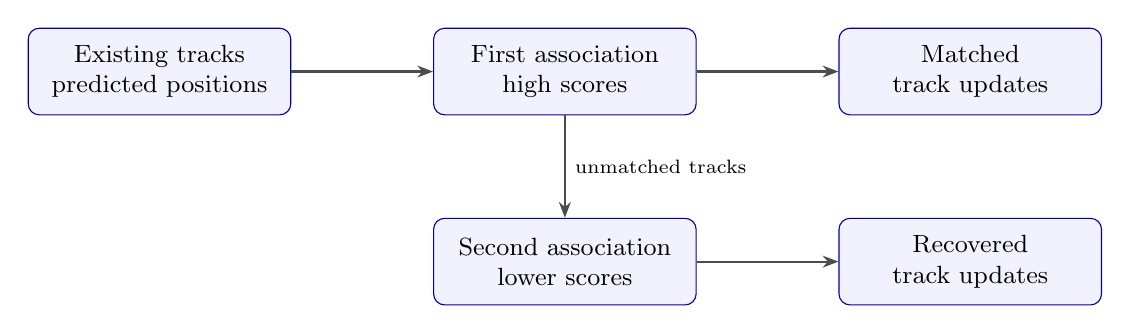
\begin{tikzpicture}[
 node distance=6mm and 6mm,
 block/.style={draw=blue!65!black,rounded corners,fill=blue!5,align=center,minimum height=11mm,text width=31mm,font=\small},
 arrow/.style={-{Stealth[length=2mm]},thick,draw=black!70}]
\node[block] (tracks) {Existing tracks\\predicted positions};
\node[block,right=18mm of tracks] (first) {First association\\high scores};
\node[block,right=18mm of first] (matched) {Matched\\track updates};
\node[block,below=13mm of first] (second) {Second association\\lower scores};
\node[block,right=18mm of second] (recover) {Recovered\\track updates};
\draw[arrow] (tracks)--(first); \draw[arrow] (first)--(matched);
\draw[arrow] (first)--node[right,font=\scriptsize]{unmatched tracks}(second);
\draw[arrow] (second)--(recover);
\end{tikzpicture}

\caption{Conceptual two-stage association: low-confidence detections can support unmatched existing tracks. The precise state transitions and thresholds are governed by the configured tracker implementation.}
\label{fig:association}
\end{figure}

Class-aware association also has consequences. The project adapter maintains separate tracker instances for detected classes and maps their internal IDs into project IDs. This avoids matching a car observation to a bus track, but an unstable detector class prediction can fragment a trajectory when a vehicle switches predicted class. A tracking experiment should therefore record the detector, class mapping, score thresholds, frame rate and tracker settings alongside HOTA or IDF1.

\subsection{BoT-SORT and camera motion}
BoT-SORT extends the family of tracking-by-detection methods with additional association mechanisms, including camera-motion compensation and optional appearance features in the original method \cite{botsort}. Camera-motion compensation estimates background motion to separate apparent object motion from camera movement. Appearance-based re-identification (ReID) can help distinguish visually different objects when geometric overlap is ambiguous.

The project configuration is tailored to fixed-camera experiments: global motion compensation is off by default, and the adapter rejects \texttt{with\_reid: true} because a ReID encoder is not integrated in the inspected version. Therefore, the mere availability of the BoT-SORT adapter should not be described as an experiment with appearance-based ReID. Enabling camera-motion compensation or incorporating ReID would require additional configuration, compute and evaluation.

\subsection{Polygon zones and the small-object problem}
A polygon zone is a region defined by vertices in image coordinates. In TrafficVision, the bottom-centre of each bounding box provides a consistent reference point for deciding whether a detection lies inside a zone. Named far, middle or near zones can use different confidence thresholds and crop strategies. A separate measurement zone can restrict speed reporting to a portion of the road where the calibration is reliable.

Zone assignment is not object detection. A polygon cannot recover a vehicle that is absent from detector predictions, nor can it independently determine a lost identity. Its contribution is to restrict or adapt the processing applied to observations. For distant traffic, a crop enlarged before inference can make small vehicles more prominent to the network, but it can also introduce duplicate boxes, larger compute requirements and missed objects at crop boundaries. A meaningful experiment would compare full-frame and crop-based processing on the same annotated frames, reporting far-zone recall, false positives and total runtime.

The coordinate frame is part of the definition: a polygon drawn on a $960\times540$ source cannot safely be reused on a differently cropped or resized frame without a verified transformation. Camera movement, video stabilization or changed optics can also invalidate a previously drawn region. These are geometric configuration issues even when the detector itself still runs.

\subsection{Homography assumptions}
If the road region is approximately planar and the camera is fixed, a homography maps a road-plane point in image coordinates to a corresponding metric point \cite{opencvhomography}. It does not map arbitrary points above the road plane correctly: roof corners, signs and elevated surfaces generally do not obey the same road-plane relation. The bottom-centre of a box is used as a practical approximation to the tire--road contact location, but an axis-aligned rectangle can move as viewpoint, occlusion or detector output changes even when the true contact point is stable.

Figure~\ref{fig:homography} illustrates the distinction between an image-space polygon and a metric road-plane coordinate system. The correspondences used to estimate $H$ must relate the same physical road points in both coordinate systems. Four point pairs are the mathematical minimum for a non-degenerate homography; more measured pairs can support a fit and a separate set of independent measurements can test it. A very low fitting error on only the four fitted points is not an independent estimate of real-world accuracy.

\begin{figure}[htbp]
\centering
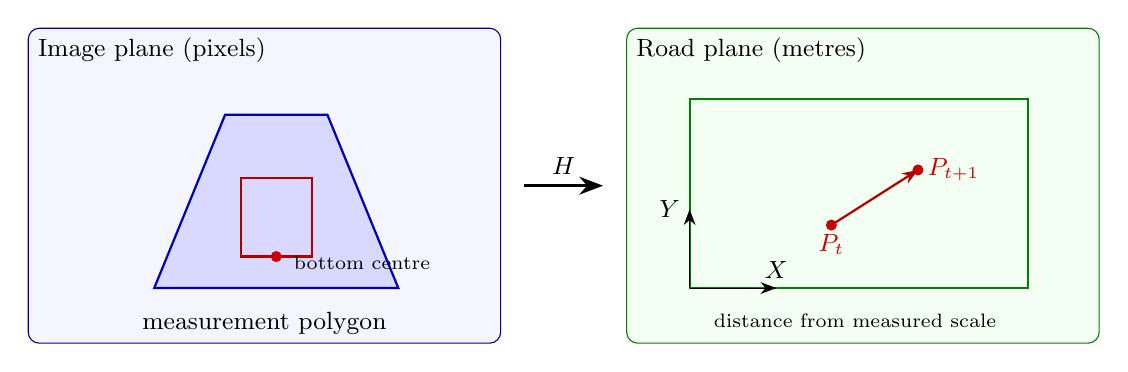
\begin{tikzpicture}[font=\small,>=Stealth]
\draw[rounded corners,fill=blue!4,draw=blue!60!black] (0,0) rectangle (6,4);
\node[anchor=north west] at (0,4) {Image plane (pixels)};
\fill[blue!15] (1.6,.7) -- (4.7,.7) -- (3.8,2.9) -- (2.5,2.9) -- cycle;
\draw[blue!70!black,thick] (1.6,.7) -- (4.7,.7) -- (3.8,2.9) -- (2.5,2.9) -- cycle;
\draw[red!70!black,thick] (2.7,1.1) rectangle (3.6,2.1);
\fill[red!80!black] (3.15,1.1) circle (2pt);
\node[anchor=west,font=\scriptsize] at (3.25,1.02) {bottom centre};
\node at (3,.25) {measurement polygon};
\draw[-{Stealth[length=3mm]},very thick] (6.3,2) -- node[above] {$H$} (7.3,2);
\draw[rounded corners,fill=green!5,draw=green!50!black] (7.6,0) rectangle (13.6,4);
\node[anchor=north west] at (7.6,4) {Road plane (metres)};
\draw[green!50!black,thick] (8.4,.7) rectangle (12.7,3.1);
\draw[-{Stealth[length=2mm]}] (8.4,.7) -- (9.5,.7) node[above] {$X$};
\draw[-{Stealth[length=2mm]}] (8.4,.7) -- (8.4,1.7) node[left] {$Y$};
\fill[red!80!black] (10.2,1.5) circle (2pt) node[below] {$P_t$};
\fill[red!80!black] (11.3,2.2) circle (2pt) node[right] {$P_{t+1}$};
\draw[-{Stealth[length=2mm]},red!70!black,thick] (10.2,1.5)--(11.3,2.2);
\node[font=\scriptsize] at (10.5,.28) {distance from measured scale};
\end{tikzpicture}

\caption{Conceptual projection from image points to road-plane coordinates. The measurement polygon selects where the estimate is used; known metric correspondences determine the scale. Geometry is illustrative, not a calibration for a real camera.}
\label{fig:homography}
\end{figure}

Writing $H=(h_{ij})$ and $w=h_{31}u+h_{32}v+h_{33}$, the projected coordinates are
\begin{equation}
 X=\frac{h_{11}u+h_{12}v+h_{13}}{w},\qquad
 Y=\frac{h_{21}u+h_{22}v+h_{23}}{w}.
\end{equation}
Near the homography horizon, $w$ approaches zero and a small image perturbation may produce a large world-coordinate displacement. An oblique or nearly horizontal view can still be used in principle, but a narrow distant road region often has little vertical resolution and is sensitive to calibration and box errors. Lens distortion, a sloped or curved road and changes in camera pose introduce further mismatch; the effective measurement area should be chosen and verified per camera.

\subsection{Uncertainty-aware Kalman speed estimator}
For each track, the project estimates a state containing two-dimensional world position and velocity:
\begin{equation}
\mathbf{x}_t=[X_t,Y_t,V_{X,t},V_{Y,t}]^{T}.
\end{equation}
Under a constant-velocity motion model over time interval $\Delta t$, the next position is predicted from the current position and velocity. The transition matrix used by the project has the form
\begin{equation}
F(\Delta t)=
\begin{bmatrix}
1&0&\Delta t&0\\
0&1&0&\Delta t\\
0&0&1&0\\
0&0&0&1
\end{bmatrix}.
\end{equation}
Predicted position covariance grows with motion uncertainty. A new observation $\mathbf z_t=[X_t,Y_t]^T$ then corrects the state when it is consistent with the prediction. The estimator checks the innovation using a Mahalanobis-distance gate, allowing outlying observations to be rejected. Excessively long gaps or repeated incompatible observations lead to a reset or reinitialization. Only observed tracks are passed to the metric update; a predicted box across a missing detection is not itself a measured world position.

The code relates pixel noise to road-plane measurement uncertainty with the homography Jacobian. For a local pixel covariance $\Sigma_{uv}$, the first-order propagated covariance is
\begin{equation}
\Sigma_{XY}\approx J_H\,\Sigma_{uv}\,J_H^T,\qquad
J_H=\frac{\partial(X,Y)}{\partial(u,v)}.
\end{equation}
The implementation uses a pixel-noise parameter and the local Jacobian to construct measurement covariance. It uses a numerically stable covariance update and checks an uncertainty criterion before displaying speed. These mechanisms express assumptions about noise; they are not a measurement of systematic error from a wrongly marked calibration or a biased bounding box.

The final estimate is the magnitude of the filtered velocity vector converted from metres per second:
\begin{equation}
\widehat v_{\mathrm{km/h}}=3.6\sqrt{V_X^2+V_Y^2}.
\end{equation}
Figure~\ref{fig:speed-filter} summarizes the dependencies of this computation. The calibration and noise assumptions are separate from the tracker identity and timing inputs.
\begin{figure}[htbp]
\centering
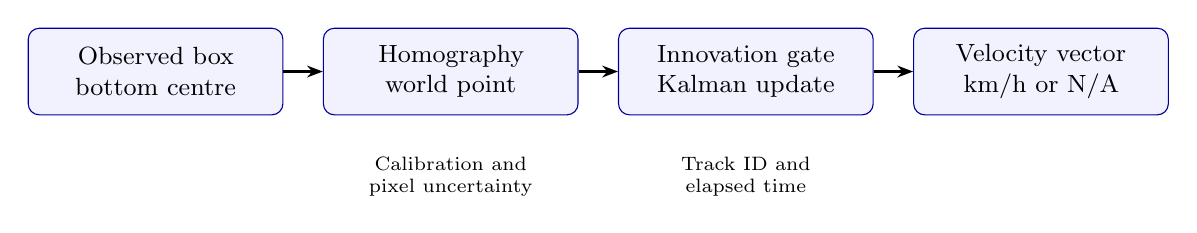
\begin{tikzpicture}[
 node distance=5mm and 5mm,
 block/.style={draw=blue!60!black,rounded corners,fill=blue!5,minimum height=11mm,align=center,text width=30mm,font=\small},
 arrow/.style={-{Stealth[length=2mm]},thick}]
\node[block] (point) {Observed box\\bottom centre};
\node[block,right=of point] (world) {Homography\\world point};
\node[block,right=of world] (gate) {Innovation gate\\Kalman update};
\node[block,right=of gate] (speed) {Velocity vector\\km/h or N/A};
\draw[arrow] (point)--(world); \draw[arrow] (world)--(gate); \draw[arrow] (gate)--(speed);
\node[font=\scriptsize,below=4mm of world,align=center] {Calibration and\\pixel uncertainty};
\node[font=\scriptsize,below=4mm of gate,align=center] {Track ID and\\elapsed time};
\end{tikzpicture}

\caption{Inputs and stages of the speed-estimation path. A numeric result requires a measured camera calibration and enough accepted observations.}
\label{fig:speed-filter}
\end{figure}
When too few reliable observations are available, calibration is missing, or a gate rejects the observation, the pipeline can report \texttt{N/A}. At a fixed frame rate, elapsed time should reflect the actual number of frames between observations; with variable-rate material, reliable presentation timestamps are preferable. A correct time interval cannot repair a misidentified vehicle after an ID switch.

\subsection{Calibration workflow and validation}
The project provides tools for selecting road points and storing image/world pairs. For a rectangular road region, the first four image points can correspond to the physical rectangle's corners, and its measured length and width supply a metric coordinate system. For an arbitrary shape, additional measured pairwise distances can reconstruct a compatible planar arrangement. A drawing tool can assist with data entry, but drawing a quadrilateral and assigning an assumed width does not measure the road. Extrapolated points outside the image should only be used when their image positions are justified independently.

A defensible workflow uses measured correspondences for the intended camera and resolution, checks for degeneracy and numerical error, and validates the estimated transformation on different known points. The measurement zone should avoid areas in which the road is hidden or the projected metric uncertainty is excessive. If the scene cannot provide adequate physical information, the system can still show detections and IDs while withholding speed. Alternative segment-speed evaluation using two road markers also requires their physical separation and the same vehicle identity at both crossing times.

\section{Evaluation Design and Interpretation}
\label{sec:evaluation-protocol}
\subsection{Why sequence-level splitting matters}
Traffic video frames are highly correlated. Two neighboring frames often contain the same cars, road background and lighting conditions. If frames from one sequence are randomly scattered between train and test, a model may encounter nearly identical scenes in both sets. This can make a frame-level test appear stronger than performance on a genuinely unseen sequence. The project therefore stores sequence IDs by split and validates that an ID is not shared across splits.

The split still needs interpretation. The published manifest lists 100 sequences, but sequence-level separation alone does not establish that every camera or physical location is independent across splits. If multiple sequences show the same location, the team should examine that relationship before claiming generalization to unseen cameras. The project also includes a 40-sequence test split; its existence is not evidence that all reported detector metrics use it. The published detection comparison is explicitly labelled validation.

\subsection{Detection matching and confusion counts}
At a given confidence threshold and IoU threshold, detection predictions can be evaluated by ordering them by confidence, matching each prediction to a previously unmatched ground-truth box of the same class, and counting successful and unsuccessful assignments. True positives (TP) are matched predictions; false positives (FP) are unmatched predictions; false negatives (FN) are ground-truth objects not matched by a qualifying prediction. The project precision/recall implementation uses this class-aware greedy matching at IoU 0.5 and confidence 0.25, after its ignore-region filtering.

\begin{equation}
\operatorname{Precision}=\frac{TP}{TP+FP},\qquad
\operatorname{Recall}=\frac{TP}{TP+FN}.
\end{equation}
Precision asks what fraction of accepted predictions are correct; recall asks what fraction of labelled objects were recovered. Lowering a confidence threshold can add true positives and false positives at the same time. A detector can achieve a high recall while making many extra predictions, as illustrated by the compact Transformer run's published fixed-threshold results. Precision and recall at one operating point do not describe the entire detector behavior.

The ignore policy also affects the counts. An ignored road area may contain unlabelled or partially annotated objects; treating every such prediction as false positive can distort the comparison. Conversely, a policy that removes too many predictions may overstate performance. TrafficVision filters predictions by whether their box centres fall in the configured ignore rectangle, with a same-class positive-match exception. This is a documented project policy and should be kept identical across the compared detectors.

\subsection{Average precision and COCO-style summaries}
Average precision (AP) summarizes a precision--recall curve obtained by changing the score threshold. AP$_{50}$ uses an IoU criterion of 0.50. The reported AP$_{50:95}$ aggregates AP at IoU thresholds from 0.50 to 0.95 in 0.05 increments using the project's TorchMetrics/COCO implementation. A higher IoU requirement demands closer spatial alignment between a predicted and a reference box. The per-class values are aggregated by the metric implementation over evaluable categories; a category with no relevant ground truth can be reported as unavailable, represented as $-1$ in the underlying records. It must not be silently treated as AP zero or as evidence of good performance for that category.

The source figure's per-epoch AP histories show why the evaluated class set matters. In the logged first and last Faster R-CNN validation epochs, the value for \texttt{others} is unavailable; the Fast R-CNN and R-CNN logs have unavailable values for \texttt{bus} and \texttt{others} in those epochs. Their per-epoch curve values therefore cannot be assumed to average over the same four-class population. This issue is independent of whether the curve values were faithfully copied from the original log files: a perfectly reproduced figure can still combine incompatible experimental quantities.

The full validation reports contain 10,260 frames for five models. The partial reports contain 400 frames for Fast R-CNN and R-CNN. Equal frame counts alone would not prove that subsets are identical, since sequence ordering and composition also matter; when possible, record exact frame IDs and a dataset manifest checksum. The current run-specific table is informative as an artifact summary, not a controlled leaderboard.

\subsection{Tracking metrics}
Tracking evaluation requires ground-truth trajectories aligned by sequence and frame. A trajectory contains identities as well as boxes, so simply counting visually distinct boxes or printed IDs on a demo cannot quantify ID switches or trajectory fragmentation. A tracker that outputs many correct boxes but repeatedly changes the identity attached to the same car may have reasonable detection quality and poor identity consistency.

The project includes an interface to TrackEval for metrics such as HOTA, IDF1 and MOTA. IDF1 summarizes identity precision and recall after associating predicted and ground-truth identities over the sequence. MOTA incorporates false positives, false negatives and identity switches relative to the number of ground-truth observations; it can be negative when errors exceed the number of reference observations. HOTA combines detection and association behavior across localization thresholds. Definitions, preprocessing and ignored-region handling must be documented before comparing scores across evaluators or benchmark leaderboards.

These are supported evaluation methods, not numerical results in the inspected artifacts. The project-specific class-aware IoU and ignore handling are not automatically equivalent to the official UA-DETRAC PR-MOTA protocol. The detector, tracker, thresholds, sequence IDs, frame range and evaluator version must accompany any future reported tracking scores.

\subsection{Speed metrics and their prerequisites}
For paired predicted and independently measured ground-truth speeds $\widehat v_i$ and $v_i$, mean absolute error (MAE) and root mean squared error (RMSE) are
\begin{equation}
\operatorname{MAE}=\frac{1}{N}\sum_{i=1}^{N}|\widehat v_i-v_i|,\quad
\operatorname{RMSE}=\sqrt{\frac{1}{N}\sum_{i=1}^{N}(\widehat v_i-v_i)^2}.
\end{equation}
Mean absolute percentage error is meaningful only where the denominator $v_i$ is nonzero; it can become unstable for very small true speeds. The report should state the unit (km/h), how speeds were synchronized, how vehicles were matched, and whether the measurements are instantaneous or averages over road segments. An error computed on mismatched vehicles or different time intervals is not a valid measure of the estimator.

Reprojection error on the four calibration correspondences is not equivalent to speed error. It measures the agreement of a fitted geometric mapping with selected points, while speed additionally depends on temporal accuracy, track identity, road-plane approximation and detector noise. Independent calibration check points and speed ground truth answer different questions and both are useful.

\subsection{Latency, memory and reproducibility}
The comparison CSV includes detector-adapter timing, parameter counts and allocated GPU memory. The evaluator times prediction calls; the resulting FPS should not be described as end-to-end video throughput when video decoding, tracking, drawing and encoding are outside that timer. A defensible runtime experiment identifies the hardware, model weights, input dimensions, batch size, precision, software versions, warm-up, synchronization policy and number of measured samples.

Experiment reproducibility also requires preserving the split, source revision, run config, initialization mode, random seed, optimizer settings, checkpoint-selection rule and exact evaluation artifacts. The report uses the recorded seed and configs without claiming multiple independent trials or statistical significance. The supplied plotting figure contains individual runs, not mean and standard deviation over repeated runs.

\section{Experiments}
\label{sec:experiments}
\subsection{Available runs and evaluation protocol}
The available artifacts contain configurations, training histories, checkpoints and detection reports for seven runs \cite{comparison,repository}. The custom-run configurations specify CUDA, seed 42, AdamW, step scheduling and gradient clipping. Selected configurations are summarised in Table~\ref{tab:training}; the configured epoch/step limits do not by themselves prove that every full dataset frame was visited in every epoch. The configurations also cap the validation batches used during custom-model training (150 for Faster R-CNN and the RT-DETR variant; 50 for Fast R-CNN and R-CNN). Thus checkpoint selection and the later evaluation reports need not use identical subsets. The YOLO native arguments record 20 epochs, batch size 16, image size 640 and AdamW, while the project's export configuration specifies a stride of five frames for the train and validation splits \cite{yoloargs,yoloconfig}. YOLO's native validation during training and the common evaluator may use different inputs and settings.

\begin{table}[htbp]
\centering
\caption{Selected published training configuration settings. Step caps apply to custom-model epochs.}
\label{tab:training}
\begin{tabular}{lrrrr}
\toprule
Run & Epochs & Batch & Learning rate & Max steps \\
\midrule
Faster R-CNN, scratch & 20 & 8 & 0.001 & 1,000 \\
Faster R-CNN, ImageNet & 15 & 8 & 0.0005 & 1,000 \\
Fast R-CNN, scratch & 10 & 2 & 0.001 & 300 \\
R-CNN, scratch & 10 & 1 & 0.001 & 200 \\
RT-DETR variant, scratch & 20 & 8 & 0.0005 & 1,000 \\
YOLOv8n, fine-tuned & 20 & 16 & 0.001 & --- \\
\bottomrule
\end{tabular}
\end{table}

Detection performance is measured with the project evaluator using COCO-style average precision (AP) at IoU 0.50 and mean AP over IoU 0.50--0.95. Precision and recall use confidence 0.25, class-aware one-to-one matching and IoU 0.50, with the ignore policy described in Section~\ref{sec:dataset}. All metrics in the published comparison CSV are labelled \texttt{val}, and no test-set result is asserted here. The evaluation script limits Fast R-CNN and R-CNN batches; the resulting reports each contain 400 frames. Other reports contain all 10,260 frames listed in the validation manifest \cite{evaluationcode,evalscript,comparison}.

\subsection{Validation detection results}
Table~\ref{tab:full} presents the five reports with the full validation frame count. The values are rounded to three decimals from the published CSV. AP depends on confidence-ranked predictions over the evaluator's thresholds, whereas the precision and recall columns are reported at a fixed confidence of 0.25. Initialization, architecture, data sampling and training budgets differ, so the table is an empirical comparison of these runs rather than a controlled ablation.

\begin{table}[htbp]
\centering
\caption{Detection reports on the 10,260-frame validation split. AP values are fractions.}
\label{tab:full}
\begin{tabular}{lrrrr}
\toprule
Run & AP$_{50}$ & AP$_{50:95}$ & Precision & Recall \\
\midrule
Faster R-CNN, scratch & 0.642 & 0.416 & 0.828 & 0.829 \\
Faster R-CNN, ImageNet & 0.719 & 0.507 & 0.736 & 0.805 \\
RT-DETR-inspired, scratch & 0.367 & 0.238 & 0.386 & 0.826 \\
YOLOv8n, COCO & 0.365 & 0.259 & 0.767 & 0.670 \\
YOLOv8n, fine-tuned & 0.750 & 0.564 & 0.825 & 0.907 \\
\bottomrule
\end{tabular}
\end{table}

The corresponding reports for Fast R-CNN and R-CNN cover only 400 validation frames (Table~\ref{tab:partial}). Both JSON files mark AP for \texttt{bus} and \texttt{others} as unavailable ($-1$), so their aggregate AP does not represent the same set of evaluable classes as the full-split reports. They are reported separately because a different number and potentially different distribution of frames invalidate a direct ranking against Table~\ref{tab:full}. They may also differ from a full-split estimate even when the same metric code is used.
\begin{table}[htbp]
\centering
\caption{Partial validation reports: 400 frames per run.}
\label{tab:partial}
\begin{tabular}{lrrrr}
\toprule
Run & AP$_{50}$ & AP$_{50:95}$ & Precision & Recall \\
\midrule
Fast R-CNN, scratch & 0.409 & 0.267 & 0.667 & 0.335 \\
R-CNN, scratch & 0.132 & 0.053 & 0.458 & 0.151 \\
\bottomrule
\end{tabular}
\end{table}

\subsection{Training curves and runtime}
The published project figure summarises training losses and per-epoch validation AP (Fig.~\ref{fig:curves}) \cite{curves}. We compared all 95 rows of its companion CSV against the original per-epoch logs and the YOLO training CSV, including the plotted loss and AP fields, within the CSV's five-decimal rounding; no field mismatch was found. The script combines distinct evaluation subsets: the recorded custom-model validation logs contain 1,200 frames per epoch for Faster R-CNN and the RT-DETR variant, 100 for Fast R-CNN and 50 for R-CNN. The YOLO series comes from its native training results on the exported validation data configured with stride five. In the first and last logged Faster R-CNN epochs, the per-class AP array reports the \texttt{others} class as unavailable ($-1$); in the corresponding Fast R-CNN and R-CNN logs, both \texttt{bus} and \texttt{others} are unavailable. The plotted values must therefore not be interpreted as performance over the same frames or the same set of evaluable classes \cite{plotcode,curveaudit}. Loss magnitudes and validation procedures are not directly comparable across architectures; YOLO's native validation is not the same artifact as the shared-evaluator results in Tables~\ref{tab:full} and \ref{tab:partial}. Curves show the recorded runs' evolution, not uncertainty across independent seeds.
\begin{figure}[htbp]
\centering
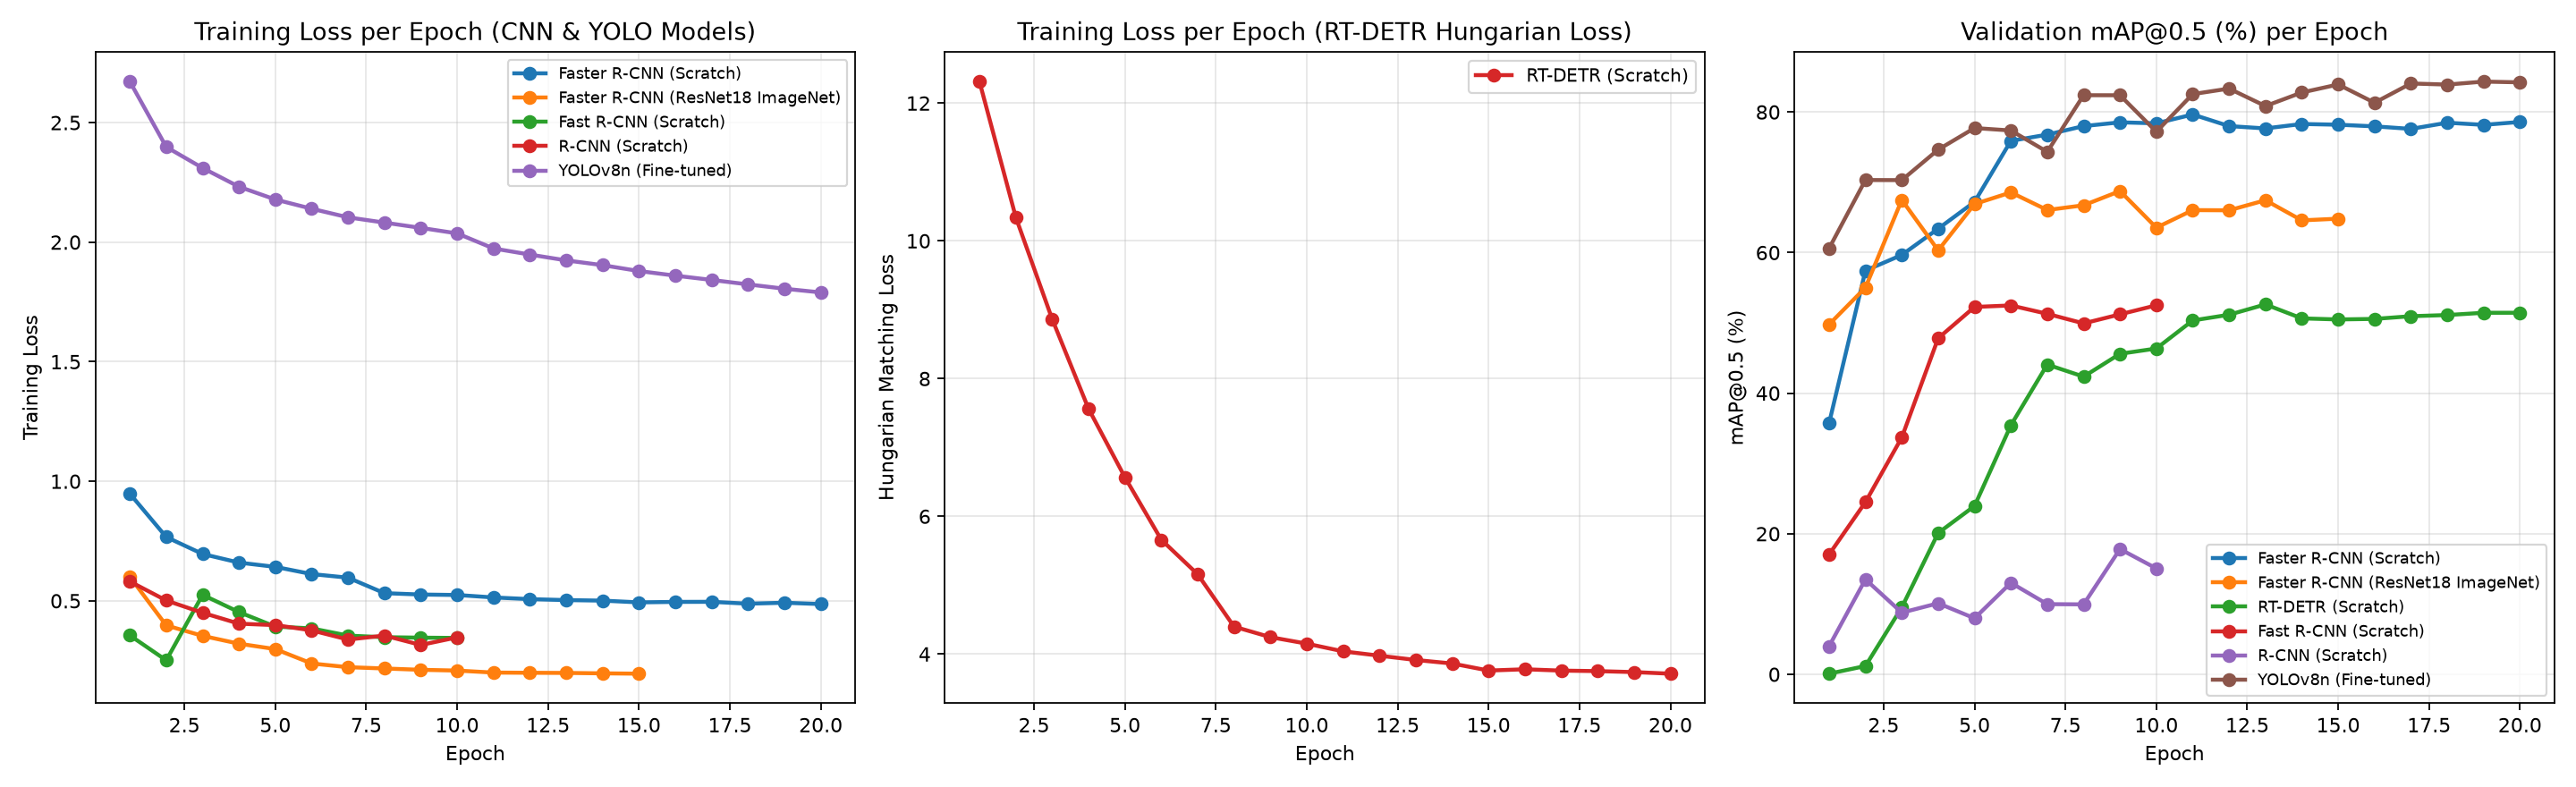
\includegraphics[width=.76\textwidth,trim=0 0 867pt 0,clip]{figures/training_loss_and_map_curves.png}
\caption{Published training losses for the R-CNN family and YOLO, enlarged from the original composite plot. The loss functions differ, so their magnitudes are not directly comparable.}
\label{fig:curves}
\end{figure}
\begin{figure}[htbp]
\centering
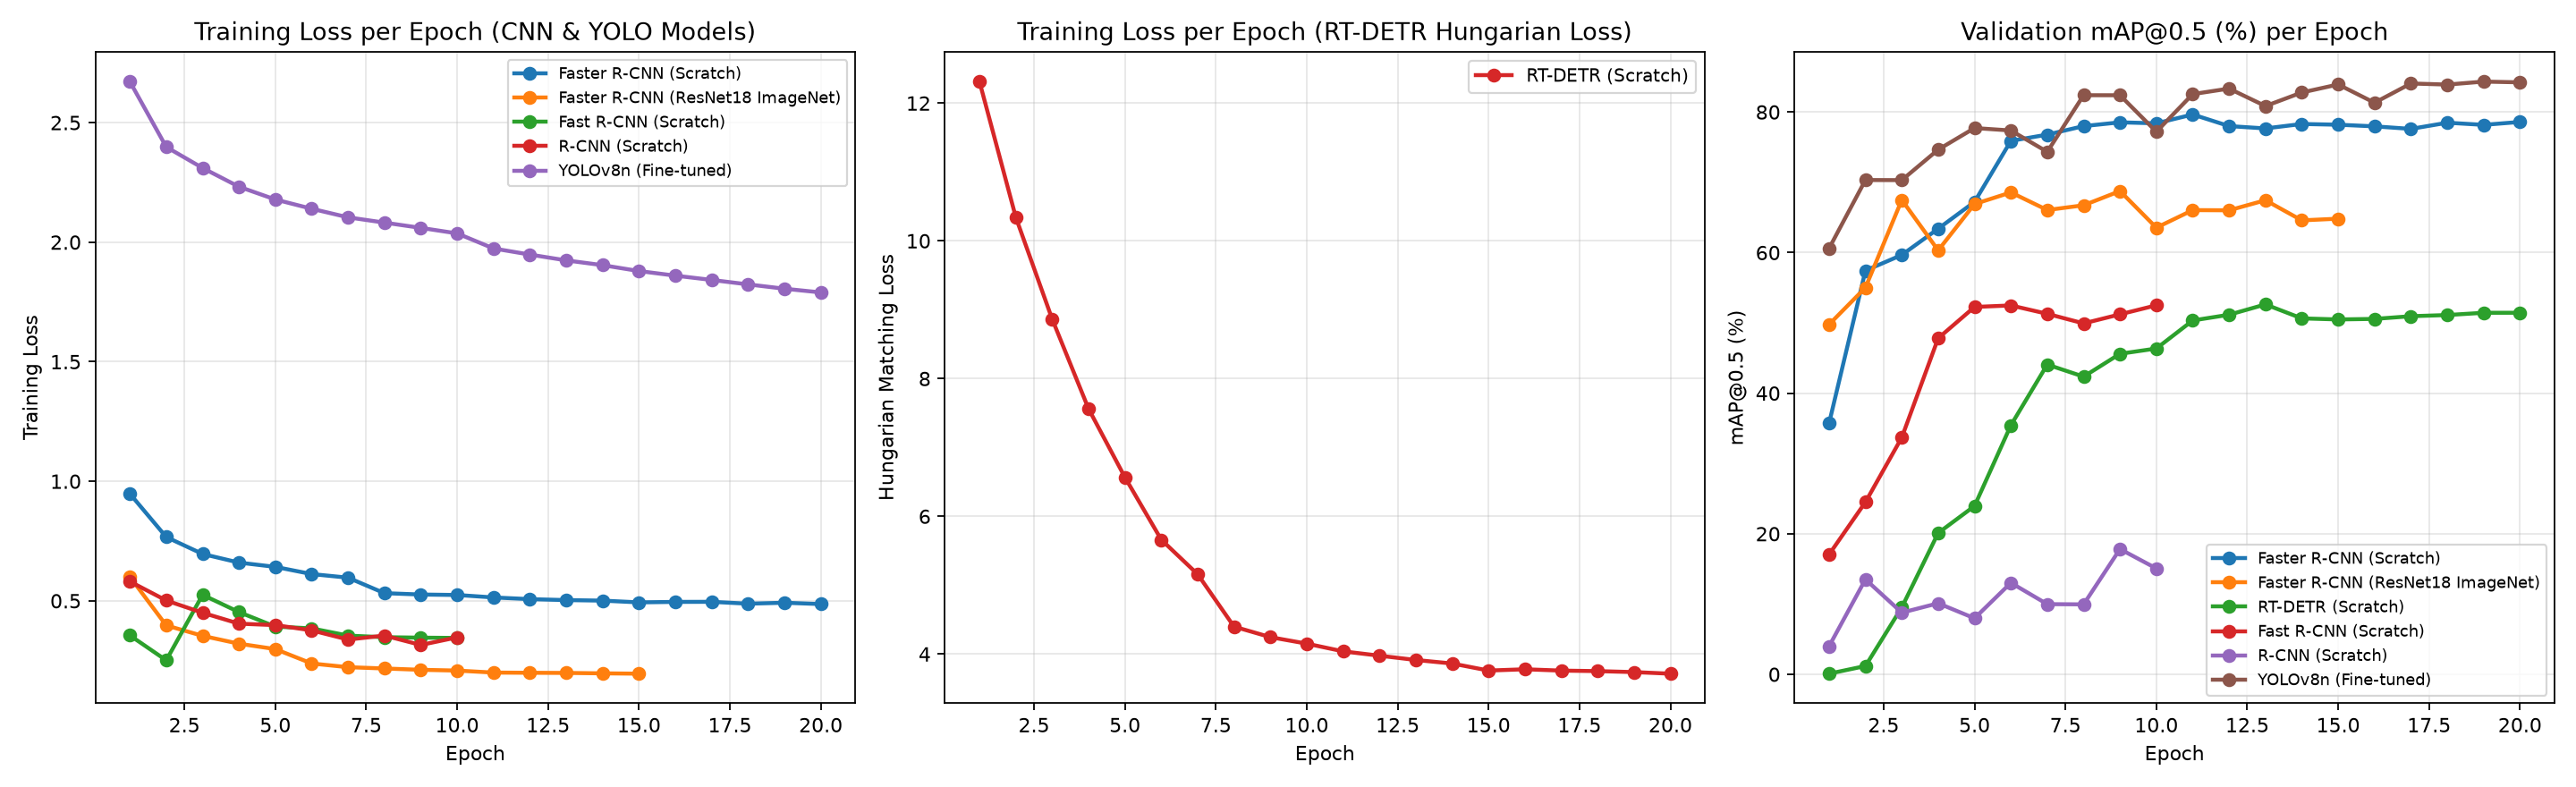
\includegraphics[width=.76\textwidth,trim=433pt 0 434pt 0,clip]{figures/training_loss_and_map_curves.png}
\caption{Published RT-DETR training loss, enlarged from the original composite plot. The original title calls it Hungarian matching loss, but the plotting script uses the total logged training loss; matching is an assignment step.}
\end{figure}
\begin{figure}[htbp]
\centering
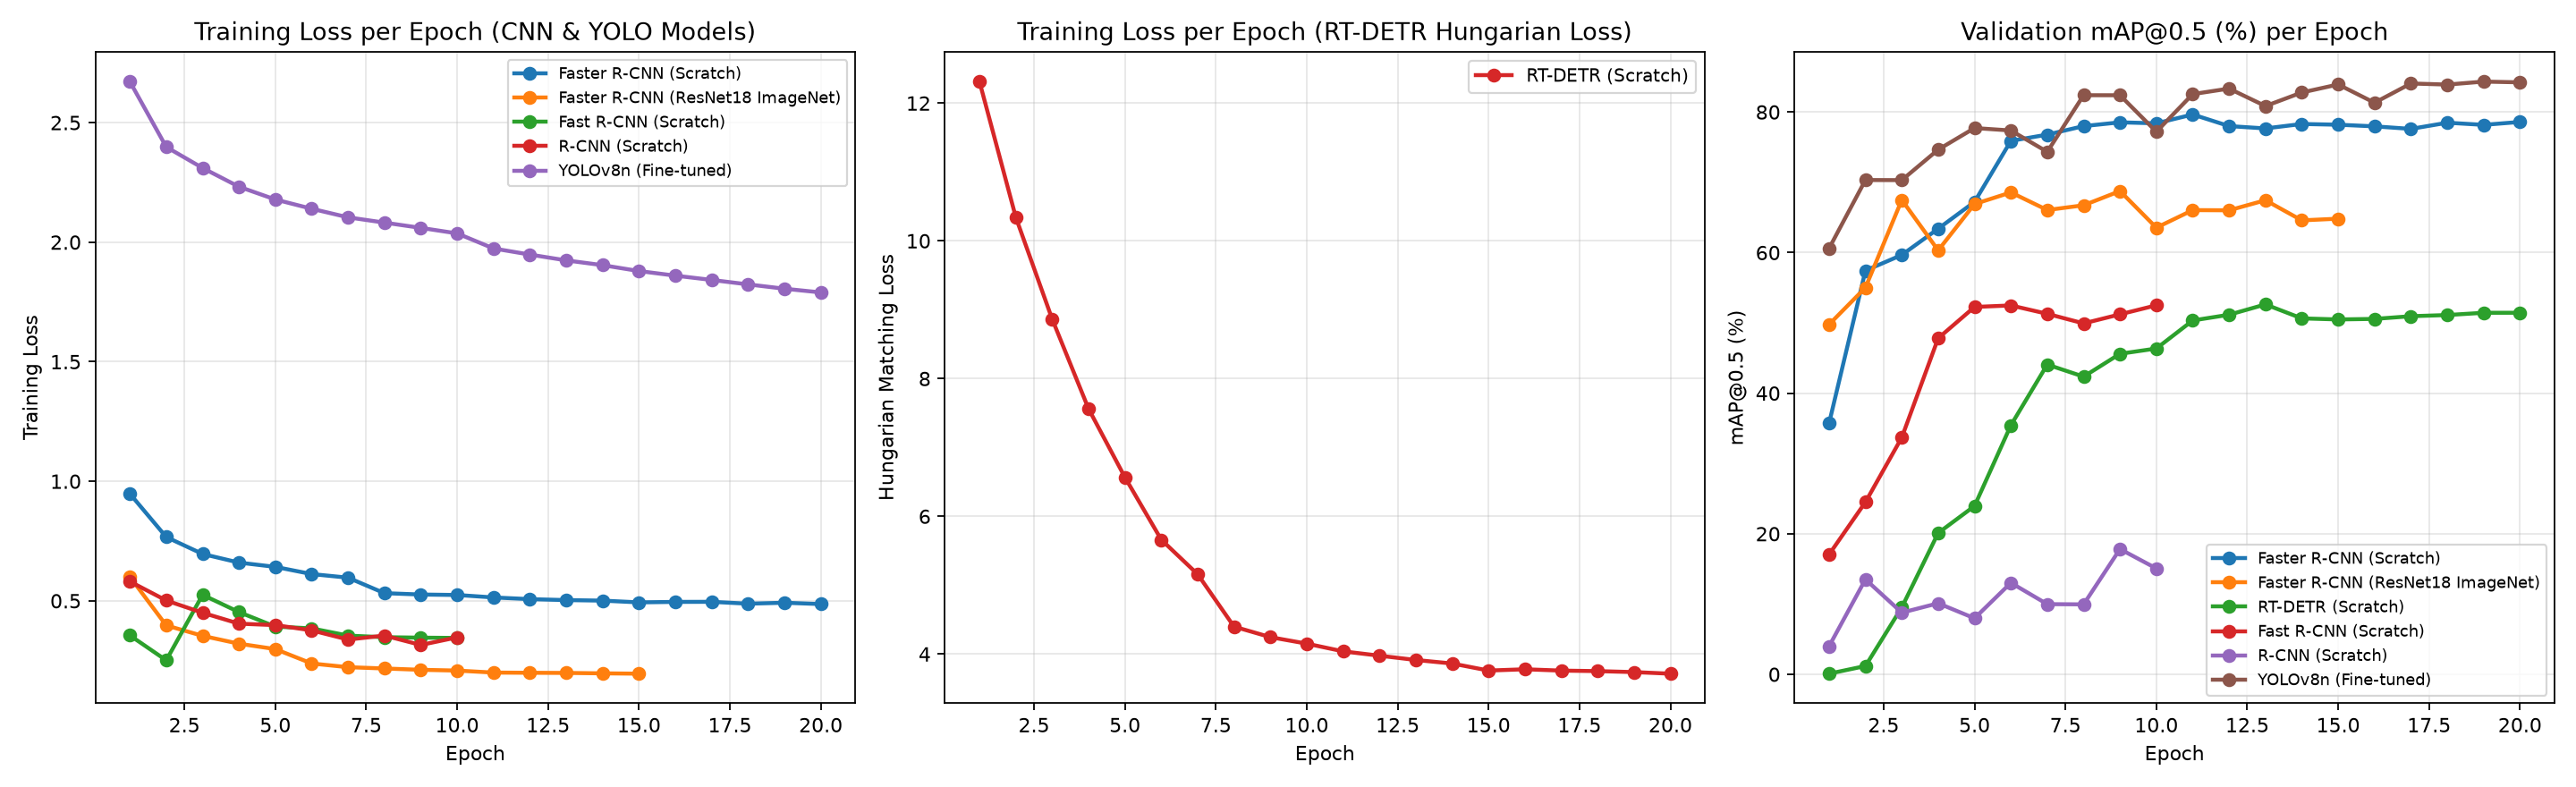
\includegraphics[width=.76\textwidth,trim=867pt 0 0 0,clip]{figures/training_loss_and_map_curves.png}
\caption{Published validation curves, enlarged from the original composite plot. The series use different numbers of frames and evaluable classes and do not constitute a common-split comparison.}
\end{figure}

The comparison file also includes prediction latency and FPS, for example 7.85 ms per image for scratch Faster R-CNN and 16.36 ms for fine-tuned YOLOv8n. The evaluator times calls to the detector adapter, not the complete decode--detect--track--render pipeline. The inspected results do not identify the GPU model or fully specify timing conditions; consequently these numbers should be treated as run-specific measurements, not general deployment or hardware-independent benchmarks \cite{evaluationcode,comparison}.

\section{Analysis of Published Experiments}
\label{sec:results-analysis}
\subsection{Reading the detection tables}
The detection tables answer a specific question: how did the available checkpoints score under the stored project-evaluation settings? They do not answer whether one architecture is intrinsically superior under equal conditions. Every full-split entry in Table~\ref{tab:full} records 10,260 validation frames, confidence threshold 0.25 for precision/recall, and the same documented ignore policy. The model configurations and initialization histories still differ substantially.

Among those five full-validation reports, fine-tuned YOLOv8n has the highest stored AP$_{50:95}$ at 0.564. The ImageNet/ResNet-18 Faster R-CNN variant records 0.507 and scratch Faster R-CNN records 0.416. The gap between the two Faster R-CNN entries is 0.091 AP points, but the backbones, parameter counts and run schedules are different. The compact RT-DETR-inspired variant records 0.238, and the COCO-only YOLOv8n baseline records 0.259. These quantities are validation observations, not confidence intervals or results on held-out test sequences.

The equal validation frame count makes these five outputs more suitable for a common table than the two 400-frame outputs. Even here, matching the total frame count does not independently prove the identities and preprocessing of every evaluated frame; the evaluation script and manifests should be archived with each run. Validation has also been used during training and model selection. As a result, the best validation checkpoint and a validation table are useful for development but should not be advertised as an unbiased final test estimate.

\subsection{Per-class analysis on the full validation set}
Table~\ref{tab:class-ap} uses the \texttt{map\_per\_class} values from the full-validation JSON files and the project mapping $1\rightarrow$ car, $2\rightarrow$ bus, $3\rightarrow$ van, $4\rightarrow$ others \cite{perclass}. These are AP$_{50:95}$ values, not AP$_{50}$. Each listed full-split JSON contains all four class IDs and finite values. Class frequency and per-sequence composition are not included in this table and must be considered before explaining differences between classes.

\begin{table}[htbp]
\centering
\caption{Per-class AP$_{50:95}$ in the five 10,260-frame validation reports.}
\label{tab:class-ap}
\begin{tabular}{lrrrr}
\toprule
Run & Car & Bus & Van & Others \\
\midrule
Faster R-CNN, scratch & 0.574 & 0.404 & 0.522 & 0.164 \\
Faster R-CNN, ImageNet & 0.549 & 0.676 & 0.512 & 0.293 \\
RT-DETR-inspired, scratch & 0.523 & 0.105 & 0.317 & 0.007 \\
YOLOv8n, COCO & 0.482 & 0.516 & 0.000 & 0.040 \\
YOLOv8n, fine-tuned & 0.636 & 0.720 & 0.534 & 0.365 \\
\bottomrule
\end{tabular}
\end{table}

The target-domain YOLO run has a higher stored value than the COCO-only baseline for every listed target class, but the zero van AP of the COCO baseline reflects the absence of an equivalent output mapping. It should not be interpreted as proof that a van was never physically detected as another COCO class. The \texttt{others} class is relatively weak in every full-validation run; however, its meaning depends on the underlying annotations and the model's class mapping. The table alone cannot distinguish class imbalance, visual ambiguity, annotation uncertainty and detector limitations.

The 400-frame Fast R-CNN and R-CNN reports list $-1$ for bus and others. This is an unavailable value in the metric output, not an AP of zero; their AP summary is therefore not a four-class aggregate over the same class population as the full reports. Both the smaller sample and missing evaluable categories are reasons to place them in a separate table. The exact sample identities should be preserved if this partial evaluation is reproduced.

\subsection{Analysis by object size}
The full-validation reports include COCO-style AP summaries for small, medium and large objects. Table~\ref{tab:size-ap} transcribes the available values. These size categories use the evaluator's annotation-area conventions; they are not automatically equivalent to manually drawn far, middle and near polygons. An object in a far zone may be small, but mapping between the two definitions must be measured.

\begin{table}[htbp]
\centering
\caption{AP$_{50:95}$ by evaluator object-size category, 10,260-frame validation reports.}
\label{tab:size-ap}
\begin{tabular}{lrrr}
\toprule
Run & Small & Medium & Large \\
\midrule
Faster R-CNN, scratch & 0.232 & 0.477 & 0.473 \\
Faster R-CNN, ImageNet & 0.056 & 0.498 & 0.645 \\
RT-DETR-inspired, scratch & 0.080 & 0.278 & 0.322 \\
YOLOv8n, COCO & 0.085 & 0.215 & 0.347 \\
YOLOv8n, fine-tuned & 0.419 & 0.542 & 0.670 \\
\bottomrule
\end{tabular}
\end{table}

Small-object AP is lower than large-object AP for every listed run, with the caveat that their category labels, training setup and prediction mapping differ. This is consistent with the practical difficulty of detecting distant vehicles, but it does not quantify the benefit of the far-zone crop path. A direct crop ablation should use the same frames, same detector checkpoint, a documented NMS policy and a validation-selected threshold, and should report both small/far recall and the increase in false positives and compute.

\subsection{What the training curves do and do not establish}
The training plot is a composite of three panels generated by the repository's aggregation script: one groups training losses for R-CNN-family and YOLO runs, one isolates the compact Transformer run's training loss, and one plots recorded validation AP$_{50}$ histories. The script reads custom-model epoch records from \texttt{metrics.jsonl}, and derives YOLO training loss by adding its recorded box, class and distribution-focal loss fields from the native results CSV \cite{plotcode}. We verified the 95 rows in the published aggregate history against those source files after rounding, with zero mismatches in the checked fields.

The original middle-panel title is misleading: despite the label ``Hungarian Matching Loss,'' the script plots the total training loss written by the trainer. Matching selects assignments, while the recorded sum also includes classification and localization losses for model outputs. The figure caption in this report corrects the interpretation without altering the group's source artifact. Moreover, the numerical magnitude of an R-CNN loss, a YOLO loss and a Transformer set loss cannot be compared as though they were measured in the same units or with identical normalizations.

The right panel has a more serious comparability limitation. Recorded custom validation sizes are 1,200 frames per epoch for both Faster R-CNN runs and the compact Transformer, 100 for Fast R-CNN and 50 for R-CNN; YOLO uses its native validation on an exported dataset configured with stride five. At least some of these small subsets do not include evaluable ground truth for all four classes. Consequently, the curves can help diagnose the evolution of an individual run but do not constitute a fair cross-model competition. In particular, the higher native YOLO per-epoch AP$_{50}$ near the end of training does not contradict its lower 0.750 full-validation AP$_{50}$ in Table~\ref{tab:full}: the two numbers come from different evaluation settings and may refer to different selected epochs.

\subsection{Training budgets and checkpoint selection}
The custom trainer caps work per epoch through \texttt{max\_steps} and caps per-epoch validation through \texttt{validation\_batches}. For example, the scratch Faster R-CNN configuration uses batch size 8 and a maximum of 1,000 optimizer steps per epoch; the Fast R-CNN configuration uses batch size 2 and 300 steps. These are upper limits on steps in the specified runs, not a guarantee that all unique frames were seen. Because the number of optimizer updates, data order and model capacity vary, similar epoch numbers cannot be equated across the table.

For custom detectors, the trainer selects a best checkpoint using the validation mAP from its configured validation process. With truncated validation, the selection signal comes from a smaller subset than the later full-validation reports. YOLO's native trainer maintains its own validation and checkpoint behavior. A future controlled study should save the precise list of frames used in checkpoint selection and final evaluation, and reserve the held-out test split for the final selected configurations. Repeated seeds and uncertainty estimates would further clarify whether observed differences are robust.

\subsection{Runtime and deployment interpretation}
The full-validation comparison records approximately 127.4 prediction calls per second for scratch Faster R-CNN, 85.9 for its ImageNet/ResNet-18 counterpart and 61.1 for fine-tuned YOLOv8n. The same CSV lists around 4.20 and 3.99 for the two partial R-CNN-family reports. These values come from the project's detector timing and depend on the execution environment. They should not be reported as the frame rate of a complete video application, nor interpreted as a universal model speed ranking across devices.

The full application has additional costs: reading and decoding frames, potentially running crop inference, performing tracking association, projecting coordinates, drawing labels and encoding video. A stronger deployment study would time the complete pipeline separately and specify whether latency is measured per image or per batch, as well as accelerator synchronization and warm-up. Memory figures should identify whether they cover only allocated model memory or a broader peak of the application. The inspected JSON provides a GPU peak allocation value, but not a complete device specification; the team should supply the actual GPU model before a quantitative systems comparison is finalized.

\subsection{What can be said about tracking and speed today}
The source contains implementations and evaluators for tracking and speed. The inspected detection results do not establish a tracking score or validate a physical speed estimate. A video with stable-looking IDs is useful qualitative evidence that a pipeline runs, but without ground-truth matching it cannot establish IDF1 or HOTA. A plotted speed value is also not proof of accuracy if the scene scale was assumed or if the camera's metric mapping was not independently checked.

The completed experiments can therefore support a substantial detector analysis now, while tracking and speed should be reported as system methodology plus clearly labelled pending quantitative validation. If the team has additional results not present in the inspected evaluation directory, those artifacts can be incorporated later with their sequence IDs, measurement protocol and ground-truth provenance.

\section{Discussion}
\label{sec:discussion}
\subsection{Detection quality and transfer learning}
Among the runs evaluated over 10,260 validation frames, fine-tuned YOLOv8n has the highest reported AP$_{50}$ and AP$_{50:95}$, followed by the ImageNet-initialized Faster R-CNN variant. This observation is limited to the published runs. The Faster R-CNN variants differ in both backbone architecture and initialization, and the YOLO experiment uses a different training pipeline and sampling configuration. The results therefore do not isolate the contribution of pretraining, architecture or training data volume.

The fine-tuned YOLOv8n AP$_{50:95}$ of 0.564 exceeds the COCO baseline's 0.259 in the reported validation evaluation. Fine-tuning is a plausible contributor, but the baseline also lacks a matching pretrained van category. The difference cannot be attributed solely to weight adaptation. The compact RT-DETR-inspired run obtains high recall at confidence 0.25 but substantially lower precision and AP, indicating that detections at that operating point contain many false positives; the result warrants inspection by class, distance and confidence rather than a claim about official RT-DETR \cite{comparison}.

\subsection{Small vehicles and measurement geometry}
The published AP for small objects differs strongly across runs: 0.419 for fine-tuned YOLOv8n, 0.232 for scratch Faster R-CNN and 0.056 for its ImageNet/ResNet-18 variant. These are evaluator categories and do not automatically correspond to a particular polygon or camera distance. Zone-specific recall, object sizes and a consistent per-sequence evaluation would be needed to quantify the proposed far-zone strategy. Similarly, confidence thresholds and crop inference affect recall and false positives and must be selected on validation data.

Oblique road views remain geometrically usable if a sufficiently visible road region is approximately planar and metric correspondences are known. Near the horizon, however, perspective amplifies image-coordinate errors; low camera angles and occlusion can make the bottom-centre of a box an unreliable proxy for road contact. A Kalman filter can model some observation noise, but it cannot correct a wrong physical scale or systematic contact-point bias. Calibration error must be measured on independent road points, and a speed claim requires ground-truth distance/time or an external speed measurement.

\subsection{Limitations and next steps}
\label{sec:limitations}
The available detection results are validation reports, not held-out test results. Fast R-CNN and R-CNN were measured on a smaller subset. Checkpoint selection, step caps and different training budgets further limit causal comparison. The training figure mixes different model losses and validation procedures, and its series should not be read as a common-scale benchmark. The available artifacts inspected for this report do not establish HOTA, IDF1, MOTA or ID switches for the final system, nor MAE/RMSE against ground-truth speed. The supplied evaluation code supports such metrics when appropriate reference data are provided; implementation is not evidence of achieved performance.

Future work should (1) run each selected detector on the same untouched test sequences, with class and ignore policies fixed; (2) evaluate tracking against trajectory IDs using the same detections and an explicitly documented protocol; (3) validate each camera's road-plane calibration and measure speed against independent ground truth; (4) benchmark latency and memory on a named device with a fixed input and timing protocol; and (5) repeat experiments with multiple seeds where feasible. Camera configuration, actual training sample counts, code revision and environment should be archived with each run.

\section{Conclusion}
TrafficVision combines vehicle detection, interchangeable tracking, polygon zones and a calibrated road-plane speed pipeline. The inspected project artifacts include detector checkpoints and validation results: fine-tuned YOLOv8n reports AP$_{50}=0.750$, while the ImageNet-initialized Faster R-CNN variant reports 0.719 over the published 10,260 validation frames. These results demonstrate functioning detector experiments but do not establish final test performance or verified physical speed accuracy. A common held-out protocol and independent camera/speed measurements are the next steps for a defensible end-to-end assessment.

\appendix
\section{Reproducibility and Artifact Audit}
\label{app:repro}
This appendix records the evidence used in the report and a practical checklist for reproducing or updating it. It does not claim to have retrained the detectors during report preparation. The reference snapshot is the Hugging Face dataset repository at commit \href{https://huggingface.co/datasets/sunnycloudhust/TrafficVision/tree/4af5adbead7219881a9c8c6a7dfa06c454d9387c}{\texttt{4af5adbe}}; the code, configurations and results cited throughout are associated with that snapshot \cite{repository}. The LaTeX report package includes small copies of the plotting script and logs used for the curve audit, not the UA-DETRAC image archives or trained checkpoints.

\subsection{Project artifact map}
\begin{table}[htbp]
\centering
\caption{Project artifacts relevant to this report. Paths are relative to the Hugging Face repository root.}
\label{tab:artifact-map}
\small
\begin{tabular}{p{0.38\textwidth}p{0.48\textwidth}}
\toprule
Artifact & Purpose \\
\midrule
\texttt{data/ua\_detrac/splits.json} & Sequence IDs for training, validation and test. \\
\texttt{data/ua\_detrac/shards.json} & Split metadata, counts, shard references and checksums. \\
\texttt{configs/experiments/} & Experiment YAMLs for custom detectors and YOLO. \\
\texttt{outputs/<run>/config.yaml} & Resolved configuration associated with a saved custom run. \\
\texttt{outputs/<run>/metrics.jsonl} & Per-epoch training loss and validation metric records. \\
\path{outputs/yolov8/train/results.csv} & Native YOLO training/validation records. \\
\texttt{outputs/evaluation/*.json} & Per-run common-evaluator reports and class/size summaries. \\
\path{outputs/evaluation/detection_comparison.csv} & Flattened summary used for Tables~\ref{tab:full} and \ref{tab:partial}. \\
\texttt{scripts/plot\_training\_curves.py} & Aggregates the source logs and draws Fig.~\ref{fig:curves}. \\
\bottomrule
\end{tabular}
\end{table}

The source report uses numeric values from files rather than from a hand-estimated reading of figure pixels. Values were rounded to three decimals in the tables. In a new version, the team should distinguish a configuration file from evidence that a run completed: a configured number of epochs is an intention, while an epoch log and a corresponding checkpoint are evidence of recorded execution. Both still need to be interpreted with the actual data sampling and evaluation code.

\subsection{Audit of the 95 curve-history rows}
The curve aggregation script names five custom log files and one YOLO results CSV. Each row of the aggregate history has a model name, epoch, training loss, validation AP$_{50}$, validation AP$_{50:95}$ and source file. For each custom log, the script converts a zero-based recorded epoch to a one-based plotting epoch and copies the logged loss and AP values. For YOLO, it reads the native epoch number, adds the three recorded training-loss components and copies native validation AP fields.

During this report review, all 95 aggregate rows were matched to their indicated original source record by epoch. The three plotted/recorded fields were checked with an absolute tolerance of $5.1\times10^{-6}$ to account for the aggregate CSV being rounded to five decimal places. No mismatching field was found. This audit establishes provenance of the numbers in the aggregate CSV and the plotting script's transformation. It does not prove that the underlying training or evaluation was error-free, that the PNG was independently regenerated, or that the curves use comparable datasets.

The validation frame counts in the custom logs are summarized in Table~\ref{tab:curve-subsets}. The negative per-class AP markers refer to unavailable category values, not negative accuracy. The table lists the values visible in the first and last recorded epochs; it should not be generalized to every epoch without reading the full logs.
\begin{table}[htbp]
\centering
\caption{Recorded custom-model per-epoch validation subsets used by the curve script.}
\label{tab:curve-subsets}
\begin{tabular}{lrl}
\toprule
Run & Frames/epoch & Unavailable classes at first/last epoch \\
\midrule
Faster R-CNN, scratch & 1,200 & Others \\
Faster R-CNN, ImageNet & 1,200 & Others \\
RT-DETR-inspired & 1,200 & Last epoch: others \\
Fast R-CNN & 100 & Bus, others \\
R-CNN & 50 & Bus, others \\
\bottomrule
\end{tabular}
\end{table}
The YOLO curve is read from its native training CSV, and the associated project configuration requests stride-five train/validation export; the exact native validation image count should be confirmed from the exported dataset or trainer logs before publication.

\subsection{Reproduction checklist for detection}
\begin{enumerate}
\item Select a fixed repository commit, install compatible Python, PyTorch, Torchvision and evaluation dependencies, and record the GPU and library versions. Confirm that CUDA is available if using the published CUDA configuration.
\item Obtain UA-DETRAC according to its distribution terms. Use the manifest, split and class mapping corresponding to the intended experiment. Confirm sequence lists, annotation coverage, image dimensions, ignored rectangles and class labels through visual inspection of sampled annotated frames.
\item Select the exact experiment YAML and initialization mode. Log the actual dataset/export size, epoch count, processed batches, seed, optimizer and model configuration. A fine-tuned checkpoint and a scratch checkpoint are distinct experimental conditions.
\item Save the checkpoint and the criterion used to select it. If validation batches are capped, save the evaluated frame IDs as well. Training-loss values with different definitions should not be interpreted on a shared absolute scale.
\item Evaluate selected checkpoints under the same evaluator, split, image preprocessing, class mapping and ignore policy. Report the number of sequences, frames and objects, including which classes have valid reference annotations.
\item Use validation data to choose thresholds and model variants. Run the final selected settings once on the held-out test split and preserve the resulting raw JSON/CSV with the code revision.
\item Repeat with independent random seeds where feasible and report the range or uncertainty. Do not infer uncertainty from a single learning curve.
\end{enumerate}

\subsection{Reproduction checklist for tracking}
Choose a set of videos with trajectory IDs and preserve frame order. Run each detector--tracker combination with recorded confidence and association thresholds. Reset tracker state between sequences; ensure predicted and reference timestamps and frame indices refer to the same underlying images. Evaluate identity-aware metrics using a consistent ignore policy and report failures such as skipped frames or missing reference IDs.

For controlled tracker comparisons, hold the detector checkpoint and detections fixed where practical. For controlled detector comparisons, hold the downstream tracker settings fixed, while acknowledging that score calibration may differ. Tracking results should report the exact combination, not only a detector or tracker name. If using the project class-aware protocol rather than the official benchmark protocol, name that protocol and avoid claiming an official leaderboard score.

\subsection{Reproduction checklist for speed}
Record the original camera resolution, frame rate or timestamp source, and any cropping, resizing or stabilization. Select a road-plane measurement zone and document camera-specific calibration points with real-world units. Fit the homography using non-degenerate correspondences, and evaluate it on independent points not used to estimate it. Avoid areas near the geometric horizon or areas where a box bottom-centre is frequently occluded.

Match speed estimates to an independent reference with a documented time interval and vehicle identity. Report the number of matched observations and excluded cases, and compute MAE/RMSE in km/h only when ground-truth speeds are available. The confidence gate, maximum allowed gap and filtering parameters affect which observations receive numeric outputs; reporting only errors on accepted tracks without reporting coverage can bias the apparent quality. Report both coverage and error, and inspect failure cases, including ID switches and camera geometry changes.

\subsection{Report-editing notes for the project team}
The author names and affiliation on the title page are placeholders because the unrelated example template does not identify this project team. Replace them with confirmed information before submission. The tables reflect the inspected snapshot and may become outdated after new experiments. The project includes configs and reference data for multiple cameras, but this report does not treat any of them as independently verified physical calibration without evidence from the team.

The validation splits and AP numbers are useful for explaining existing work, but final submission requirements may call for additional test-set and tracking results. If such artifacts exist outside the inspected repository snapshot, add their source paths, split and protocol before incorporating the numbers. A concise figure of a genuinely calibrated test scene would be valuable if the team can provide one, clearly marked with camera ID, chosen reference points and measurement provenance.

\begin{thebibliography}{99}
\bibitem{detrac} L. Wen et al., ``UA-DETRAC: A new benchmark and protocol for multi-object detection and tracking,'' \emph{Computer Vision and Image Understanding}, 193, 102907, 2020. \url{https://doi.org/10.1016/j.cviu.2020.102907}.
\bibitem{rcnn} R. Girshick et al., ``Rich feature hierarchies for accurate object detection and semantic segmentation,'' CVPR, 2014. \url{https://arxiv.org/abs/1311.2524}.
\bibitem{fast} R. Girshick, ``Fast R-CNN,'' ICCV, 2015. \url{https://arxiv.org/abs/1504.08083}.
\bibitem{faster} S. Ren et al., ``Faster R-CNN: Towards real-time object detection with region proposal networks,'' NeurIPS, 2015. \url{https://arxiv.org/abs/1506.01497}.
\bibitem{rtdetr} Y. Zhao et al., ``DETRs Beat YOLOs on Real-time Object Detection,'' CVPR, 2024. \url{https://arxiv.org/abs/2304.08069}.
\bibitem{sort} A. Bewley et al., ``Simple Online and Realtime Tracking,'' ICIP, 2016. \url{https://arxiv.org/abs/1602.00763}.
\bibitem{bytetrack} Y. Zhang et al., ``ByteTrack: Multi-Object Tracking by Associating Every Detection Box,'' ECCV, 2022. \url{https://arxiv.org/abs/2110.06864}.
\bibitem{botsort} N. Aharon et al., ``BoT-SORT: Robust Associations Multi-Pedestrian Tracking,'' 2022. \url{https://arxiv.org/abs/2206.14651}.
\bibitem{yolo} Ultralytics, ``Ultralytics YOLO documentation.'' \url{https://docs.ultralytics.com/}.
\bibitem{opencvhomography} OpenCV, ``Basic concepts of the homography.'' \url{https://docs.opencv.org/4.x/d9/dab/tutorial_homography.html}.
\bibitem{repository} TrafficVision Project Team, ``TrafficVision project artifacts,'' Hugging Face Dataset repository, accessed 27 November 2026. \url{https://huggingface.co/datasets/sunnycloudhust/TrafficVision/tree/4af5adbead7219881a9c8c6a7dfa06c454d9387c}.
\bibitem{manifest} TrafficVision Project Team, ``Shard manifest and split counts,'' accessed 27 November 2026. \url{https://huggingface.co/datasets/sunnycloudhust/TrafficVision/blob/4af5adbead7219881a9c8c6a7dfa06c454d9387c/data/ua_detrac/shards.json}.
\bibitem{comparison} TrafficVision Project Team, ``Detection comparison,'' accessed 27 November 2026. \url{https://huggingface.co/datasets/sunnycloudhust/TrafficVision/blob/4af5adbead7219881a9c8c6a7dfa06c454d9387c/outputs/evaluation/detection_comparison.csv}.
\bibitem{architecture} TrafficVision Project Team, ``Architecture notes,'' accessed 27 November 2026. \url{https://huggingface.co/datasets/sunnycloudhust/TrafficVision/blob/4af5adbead7219881a9c8c6a7dfa06c454d9387c/docs/ARCHITECTURE.md}.
\bibitem{evaluationcode} TrafficVision Project Team, ``Detection evaluator source,'' accessed 27 November 2026. \url{https://huggingface.co/datasets/sunnycloudhust/TrafficVision/blob/4af5adbead7219881a9c8c6a7dfa06c454d9387c/src/trafficvision/evaluation/detection_metrics.py}.
\bibitem{evalscript} TrafficVision Project Team, ``Detector evaluation script,'' accessed 27 November 2026. \url{https://huggingface.co/datasets/sunnycloudhust/TrafficVision/blob/4af5adbead7219881a9c8c6a7dfa06c454d9387c/scripts/evaluate_all_detectors.py}.
\bibitem{rtdetrcode} TrafficVision Project Team, ``Compact Transformer detector source,'' accessed 27 November 2026. \url{https://huggingface.co/datasets/sunnycloudhust/TrafficVision/blob/4af5adbead7219881a9c8c6a7dfa06c454d9387c/src/trafficvision/models/detectors/rtdetr/model.py}.
\bibitem{yoloconfig} TrafficVision Project Team, ``YOLO training configuration,'' accessed 27 November 2026. \url{https://huggingface.co/datasets/sunnycloudhust/TrafficVision/blob/4af5adbead7219881a9c8c6a7dfa06c454d9387c/outputs/yolov8/config.yaml}.
\bibitem{yoloargs} TrafficVision Project Team, ``YOLO native training arguments,'' accessed 27 November 2026. \url{https://huggingface.co/datasets/sunnycloudhust/TrafficVision/blob/4af5adbead7219881a9c8c6a7dfa06c454d9387c/outputs/yolov8/train/args.yaml}.
\bibitem{curves} TrafficVision Project Team, ``Training loss and validation curves,'' accessed 27 November 2026. \url{https://huggingface.co/datasets/sunnycloudhust/TrafficVision/blob/4af5adbead7219881a9c8c6a7dfa06c454d9387c/outputs/evaluation/training_loss_and_map_curves.png}.
\bibitem{plotcode} TrafficVision Project Team, ``Training curve aggregation script,'' accessed 27 November 2026. \url{https://huggingface.co/datasets/sunnycloudhust/TrafficVision/blob/4af5adbead7219881a9c8c6a7dfa06c454d9387c/scripts/plot_training_curves.py}.
\bibitem{curveaudit} TrafficVision Project Team, ``Training loss history and source-file index,'' accessed 27 November 2026. \url{https://huggingface.co/datasets/sunnycloudhust/TrafficVision/blob/4af5adbead7219881a9c8c6a7dfa06c454d9387c/outputs/evaluation/training_loss_history.csv}.
\bibitem{perclass} TrafficVision Project Team, ``Per-run detection evaluation reports,'' accessed 27 November 2026. \url{https://huggingface.co/datasets/sunnycloudhust/TrafficVision/tree/4af5adbead7219881a9c8c6a7dfa06c454d9387c/outputs/evaluation}.
\end{thebibliography}

\end{document}
